\documentclass{beamer}

\usetheme{Frankfurt}
%\usetheme{Warsaw}

%\usepackage{ragged2e}
\usepackage{graphicx}

\usepackage[justification=centering]{caption}

\usepackage{rotating}

\usepackage{amsmath}
\usepackage{amssymb}
\usepackage{yquant}
\usetikzlibrary{fit, quotes}
\usetikzlibrary{snakes,arrows,shapes}

\usepackage{graphicx}

\usepackage{float}
\usepackage{hyperref}
\usepackage{physics}
\def\be#1\ee{\begin{equation}#1\end{equation}}

\usepackage[utf8]{inputenc}

%\usepackage{color}
\usepackage[dvipsnames]{xcolor}

\renewcommand{\mark}			{{\bf Oznaczenie: \\}}
\renewcommand{\det}[1]			{det \left( #1 \right)}
\renewcommand{\ker}[1]			{ker \left( #1 \right)}
\renewcommand{\limits}[1]		{\left. #1 \right|}
\renewcommand{\d}				{\delta}
\newcommand{\tg}[2]			{tg^{#1}\parenthesis{#2}}
\newcommand{\ctg}[2]			{ctg^{#1}\parenthesis{#2}}

\newcommand{\im}[1]				{Im \left( #1 \right)}
\newcommand{\task}[1]			{{\bf Zadanie #1.}\\}
\newcommand{\observation} 		{{\bf Obserwacja:}\\}
\newcommand{\property}[1] 		{{\bf Własności } #1 :\\ }
\newcommand{\theoremName}[1]	{{\bf Twierdzenie (#1):}}
\newcommand{\conclusion}		{{\bf Wniosek:}}
\newcommand{\remark}			{{\bf Uwaga:\\}}
\newcommand{\question}			{{\bf Pytanie:\\}}
\newcommand{\mb}[1] 			{\mathbb{#1}}
\newcommand{\mc}[1]				{\mathcal{#1}}
\newcommand{\ilim}[1]			{lim_{#1 \to \infty}}
\newcommand{\zlim}[1]			{lim_{#1 \to 0}}
\newcommand{\pdiv}[2]			{\frac{\partial #1}{\partial #2}}
\newcommand{\dive}[2]			{\frac{d #1}{d #2}}
\newcommand{\pdivpt}[3]			{\left. \frac{\partial #1}{\partial #2} \right|_{#3}}
\newcommand{\ndimfunc}[1]		{\left\{ 
	\begin{array}{ll}
		#1
	\end{array}
	\right.}
\newcommand{\colvec}[1]			{\left[
	\begin{array}{c}
		#1
	\end{array}
	\right]}
\newcommand{\rowvec}[1]			{\left[
	#1
	\right]}
\newcommand{\cmatrix}[2]		{\left[
	\begin{array}{#1}
		#2
	\end{array}
	\right]}
\newcommand{\parenthesis}[1]	{\left( #1 \right)}
\newcommand{\brackets}[1]		{\left\{ #1 \right\}}
\newcommand{\linSys}[1]			{
	\left\{ 
	\begin{array}{l}
		#1
	\end{array} 
	\right.
}
\newcommand{\e}					{\epsilon}
\renewcommand{\d}				{\delta}
\renewcommand{\a}				{\alpha}
\renewcommand{\b}				{\beta}
\newcommand{\lin}[1]			{\left< #1 \right>}
\newcommand{\sprod}[2]			{\left< \left. #1 \right| #2 \right> }
\newcommand{\x}					{\times}
\newcommand{\subs}[1]			{
	\left/ \left/
	\begin{array}{l}
		#1
	\end{array}
	\right/ \right/
}
\newcommand{\ver}[1]			{\hat{e}_{#1}}
\newcommand{\p}[1]				{\partial_{#1}}
\newcommand{\tdiv}				{\frac{d}{dt}}

\newcommand\blfootnote[1]{%
  \begingroup
  \renewcommand\thefootnote{}\footnote{#1}%
  \addtocounter{footnote}{-1}%
  \endgroup
}

\usepackage{physics}

\newcommand{\gcm}{{\color{OliveGreen} \checkmark}}
\newcommand{\rx}{{\color{red} $\times$}}

% Define custom colors
\definecolor{codeblue}{rgb}{0.25,0.5,0.75}
\definecolor{backgray}{rgb}{0.95,0.95,0.95}

\usepackage{listings}
% Python code style
\lstdefinestyle{pythonstyle}{
	language=Python,                 % Use Python language
	backgroundcolor=\color{backgray}, % Set background color
	commentstyle=\color{OliveGreen},       % Comments in green
	keywordstyle=\color{blue},        % Keywords in blue
	stringstyle=\color{codeblue},     % Strings in light blue
	basicstyle=\ttfamily\footnotesize,% Basic font style
	frame=single,                     % Frame the code
	breaklines=true,                  % Allow breaking lines
	numbers=left,                     % Line numbers on the left
	numberstyle=\tiny\color{gray},    % Line number style
	tabsize=4,                        % Set tab size to 4 spaces
	showstringspaces=false,            % Do not show spaces in strings
	morekeywords = {QMLModel, ModelFinder}
}
\lstset{style=pythonstyle}





\usepackage{amsmath,epsfig,mathrsfs,graphicx,amssymb,color,float}
\usepackage[T1]{fontenc}
\usepackage{t1enc}
\usepackage{hyperref}
\usepackage{array}
\usepackage{booktabs}
\usepackage{ulem}

\newcommand{\h}[1]{\hat{ #1}}
\newcommand{\f}[2]{\frac {#1}{#2}}
\def\e{\boldsymbol e}
\def\p{\partial}
\newcommand{\g}[1]{{\boldsymbol #1}}
\def\rmd{\mathrm d}
\def\rmi{\mathrm i}
\def\rme{\mathrm e}
\def\be#1\ee{\begin{equation}#1\end{equation}}
\newcommand{\ba}{\begin{eqnarray} }
	\newcommand{\ea}{\end{eqnarray} }
\def\cor#1{{\color{red}#1}}
\def\kor#1{{\color{blue}#1}}



\usepackage{amsmath,epsfig,mathrsfs,graphicx,amssymb,color,float}
\usepackage[T1]{fontenc}
\usepackage{t1enc}
\usepackage{hyperref}
\usepackage{array}
\usepackage{booktabs}
\usepackage{ulem}


\def\e{\boldsymbol e}
\def\p{\partial}
\def\rmd{\mathrm d}
\def\rmi{\mathrm i}
\def\rme{\mathrm e}
\def\be#1\ee{\begin{equation}#1\end{equation}}
\def\cor#1{{\color{red}#1}}
\def\kor#1{{\color{blue}#1}}



%PAKIETY
%\usepackage[cp1250]{inputenc}   % pozwala wprowadza��„�¢Â€Â¡ polskie znaki bezpo�„¹�¢Â€Âºrednio z klawiatury
\usepackage{amsmath}            % AMS-LaTeX (AMS-Math)
\usepackage{amsfonts}           % ekstra fonty matematyczne
\usepackage{amssymb}            % ekstra symbole matematyczne
%\usepackage{a4wide}             % szersza kolumna tekstu ni�„¹�„½ domy�„¹�¢Â€Âºlnie
\usepackage{enumerate,graphicx}
%\usepackage{multicol}
\usepackage{array}
\usepackage{booktabs}
\usepackage{bbm}
\usepackage{physics}

%PAKIETY
%\usepackage{polski}             % spolszczenie LaTeXa
%\usepackage[utf8]{inputenc}   % pozwala wprowadza�¦ polskie znaki bezpoœrednio z klawiatury
\usepackage{amsmath}            % AMS-LaTeX (AMS-Math)
\usepackage{amsfonts}           % ekstra fonty matematyczne
\usepackage{amssymb}            % ekstra symbole matematyczne
% szersza kolumna tekstu ni¿ domyœlnie
\usepackage{enumerate,graphicx}
\usepackage{array}
\usepackage{booktabs}
\usepackage{yquant}
\usetikzlibrary{fit, quotes}
\usetikzlibrary{snakes,arrows,shapes}
\useyquantlanguage{groups}
\usepackage{physics}
\usepackage{todonotes}
\newtheorem{thm}{Theorem}





\setbeamersize{text margin left=5mm,text margin right=5mm} 

\def\arraystretch{1.5} % Rozciąga wysokość tablicy

\setbeamertemplate{navigation symbols}{} % remove navigation symbols

\title[\tiny Testing Leggett-Garg inequalities]{Testing time order Leggett-Garg inequalities with weak measurements on contemporary quantum computers}

\author[Tomek Rybotycki]{\textbf{Tomek Rybotycki}}
\institute[SRI PAS]{
	Systems Research Institute, Polish Academy of Sciences\\
	Nicolaus Copernicus Astronomical Center, Polish Academy of Sciences\\
	Center of Excellence in Artificial Intelligence, AGH University of Cracow
}

\date{
	\includegraphics[height=1cm]{figs/logos/cqt_logo.pdf}\\
	CQT Talk\\
	11 VII 2025, Singapore
}
\logo{
	
\includegraphics[height=1cm]{figs/logos/ibs_pan_CMYK.pdf}
	
\includegraphics[height=1cm]{figs/logos/camk.pdf}
	
\includegraphics[height=1cm]{figs/logos/ceai-logo-icon.png}
}


\begin{document}
	
	%\justifying
	
	\frame{\titlepage}
	
	\section{Introduction}
	
	\begin{frame}{Joint work with}
	\vspace{-1cm}
	\begin{figure}
		\includegraphics[height=3cm]{figs/bednorz.jpg}
		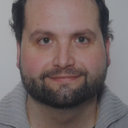
\includegraphics[height=3cm]{figs/josep.jpg}
		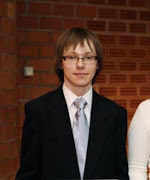
\includegraphics[height=3cm]{figs/bzglinicki.jpg}
		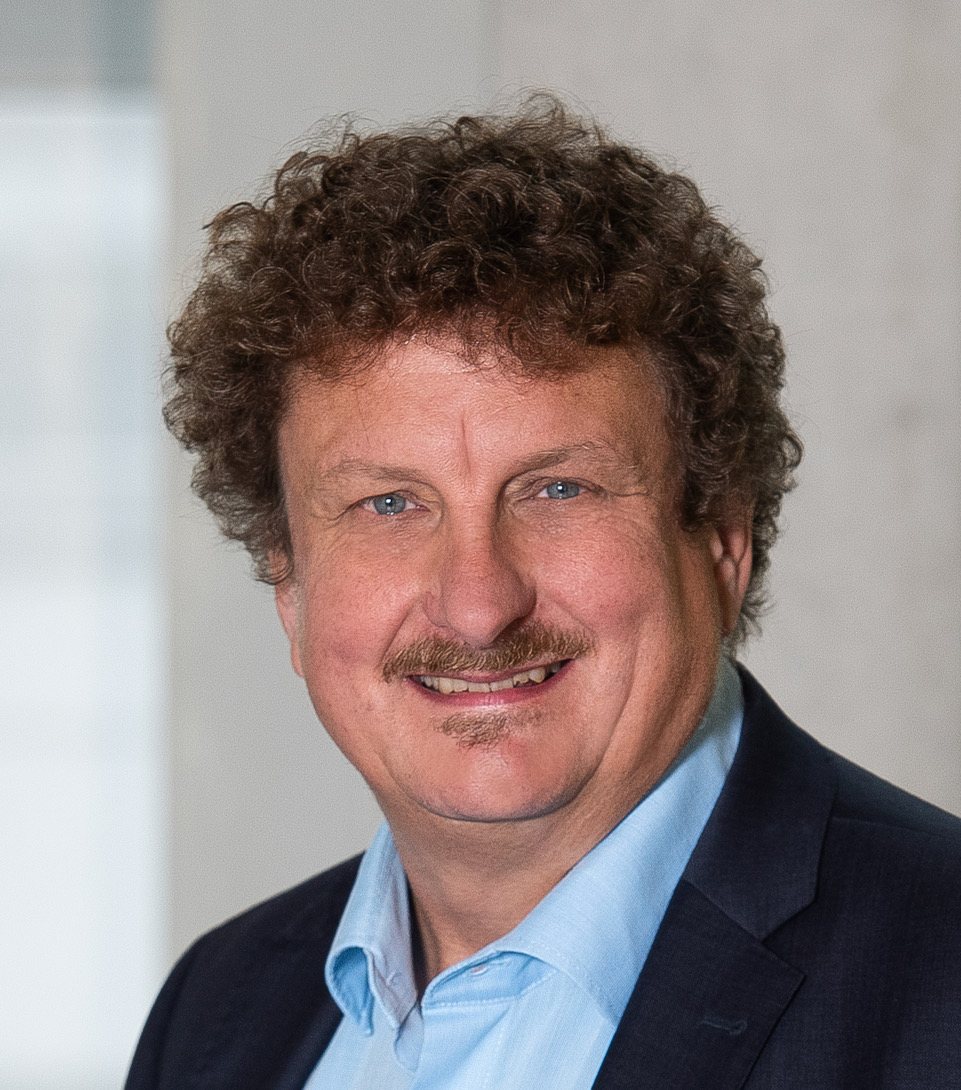
\includegraphics[height=3cm]{figs/WolfgangBelzig.jpeg}
	\end{figure}
	
		\begin{columns}
		\begin{column}{0.5\textwidth}
			
			\begin{enumerate}
				
				\item Adam Bednorz
				
				\item Tomasz Bia{\l}ecki
				
				\item Josep Batle
				
			\end{enumerate}
			
		\end{column}
		
		\begin{column}{0.5\textwidth}
			
			\begin{enumerate}
				
				\item Adam Szereszewski
				
				\item Bart{\l}omiej Zglinicki
				
				\item Wolfgang Belzig
				
			\end{enumerate}
			
		\end{column}
	\end{columns}
	
	\end{frame}
	
	\begin{frame}{About the work}
		
		\begin{columns}
			\begin{column}{0.5\textwidth}
				
				\begin{enumerate}
					
					\item Part of the QC benchmarking publication series.
					
					\item Testing complementary (to the previous work) kind of behavior.
					
					\item First time experiments connecting time-related (in)equalities and weak measurements.
					
					\item Another step towards QC benchmarking suite\footnote{Work in progress.}.
					
				\end{enumerate}
				
			\end{column}
			
			\begin{column}{0.5\textwidth}
				
				\begin{figure}
					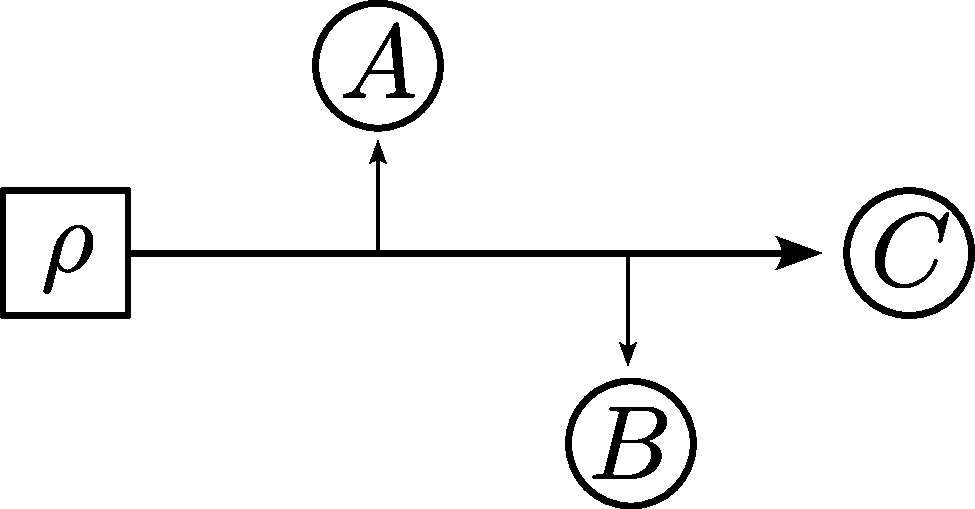
\includegraphics[scale=.3]{figs/wABC.pdf}\\
					\medskip
					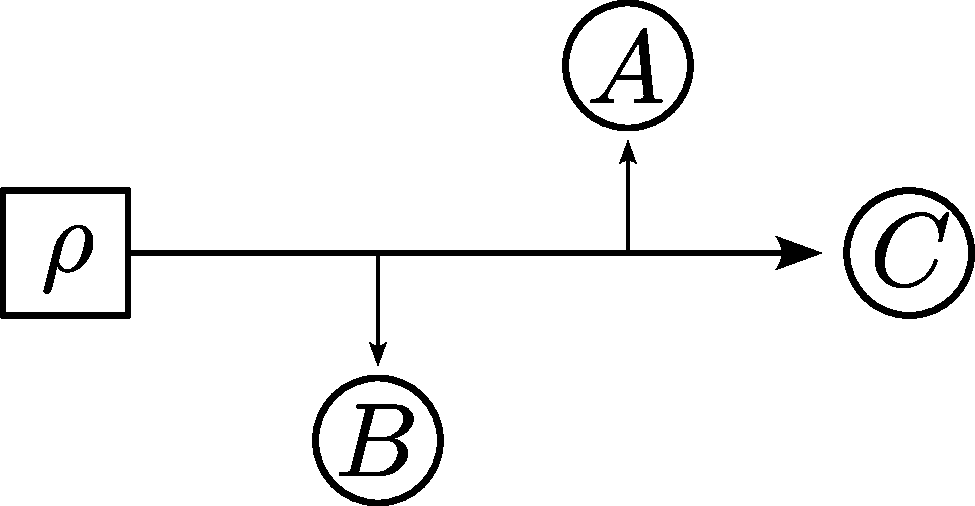
\includegraphics[scale=.3]{figs/wBAC.pdf}
				\end{figure}
				\vspace{1cm}
				
				
			\end{column}
		\end{columns}
		
	\end{frame}
	
	\begin{frame}{Agenda}
	
	\vspace{-1cm}
	\begin{columns}
		\begin{column}{0.5\textwidth}
			
			\begin{enumerate}
			
				\item Introduction
				\begin{enumerate}
					\item Motivation
					\item LG inequality
					\item Time order equality
					\item Weak measurements
				\end{enumerate}
				
				\item Experiments
				\begin{enumerate}
					\item high-level idea
					\item Protocol I
					\item Protocol II
				\end{enumerate}
				
				\item Results
				\begin{enumerate}
					\item LG on IBM
					\item Time order on IBM
					\item LG and time order on IonQ
				\end{enumerate}
				
				\item Conclusions
				
			
			\end{enumerate}
			
		\end{column}
		
		\begin{column}{0.5\textwidth}

			\begin{figure}
				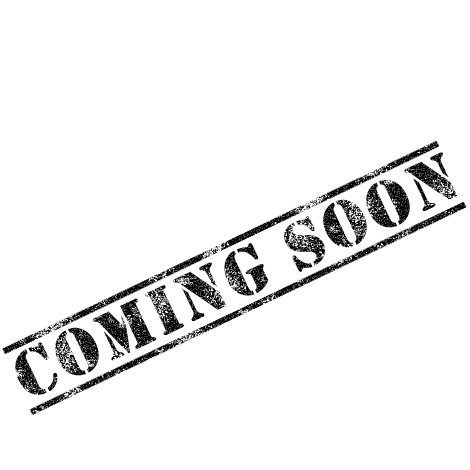
\includegraphics[width=\textwidth]{figs/coming-soon.png}
				\caption{Source: \hyperref[https://upload.wikimedia.org/wikipedia/commons/8/80/Comingsoon.png]{Wiki.}}
				\vspace{1cm}
			\end{figure}
			

		\end{column}
	\end{columns}
	
	\end{frame}
	
%%%%%%%%%%%%%%%%%%%%%%%%%%%%%%%%%%

	\begin{frame}{Motivation}
		
		\vspace{-0.5cm}
		\begin{columns}
			\begin{column}{0.5\textwidth}
				
				\begin{figure}
					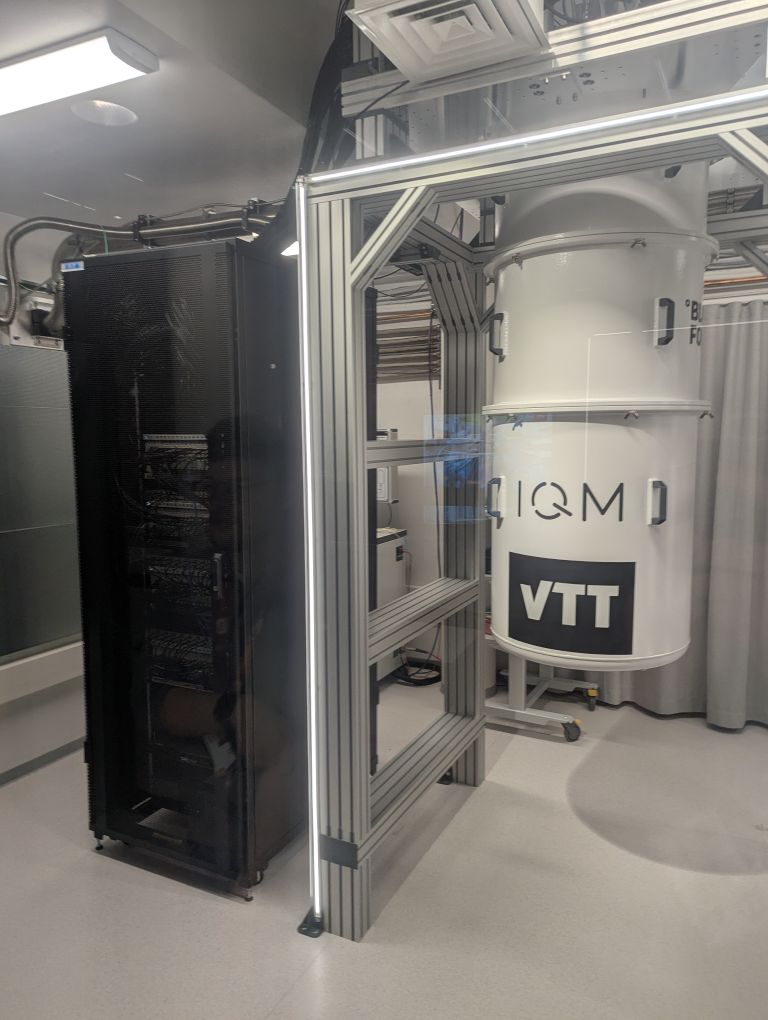
\includegraphics[width=\textwidth]{figs/IQM.jpg}
				\end{figure}
				
			\end{column}
			
			\begin{column}{0.5\textwidth}
				
				\begin{enumerate}
					\item Growing number of NISQ devices.
					\item Some limitations of the contemporary QCs are not well known.
					\item We need to benchmark QCs to know what can be done with them.
					\item LG requires noninvasiveness. Weak measurements are currently the best candidates for that.
				\end{enumerate}
				
				
			\end{column}
		\end{columns}
		
	\end{frame}
	
	\begin{frame}{Leggett-Garg inequalities}
		
		\begin{columns}
			\begin{column}{0.5\textwidth}
				
				Suppose we have a single system and three observables, $A$, $B$, $C$ with at least one
				of them measured noninvasively. Then, assuming the mapping of
				the measurement outcomes, $A\to a$, $B\to b$, $C\to c$, the correlations
				$\langle a\rangle$, $\langle ab\rangle$, or $\langle abc\rangle$ reflect the properties
				of some underlying probability distribution $p(a,b,c)$. If $|a|,|b|\leq 1$ then the
				LG inequality holds
				\be
				\langle  a\rangle+\langle  b\rangle-\langle  a b\rangle\leq 1.
				\ee
			
			\end{column}
			
			\begin{column}{0.5\textwidth}
				
				\begin{figure}
					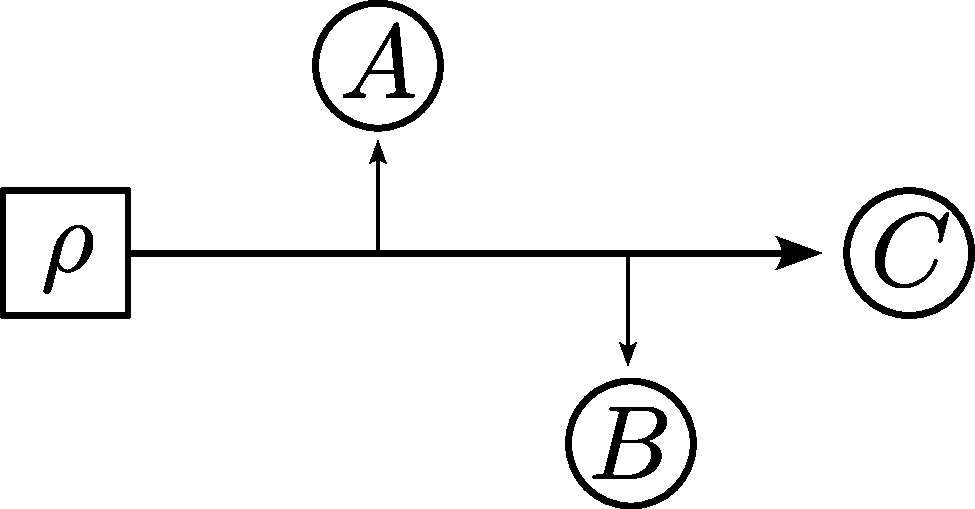
\includegraphics[scale=.3]{figs/wABC.pdf}\\
					\medskip
					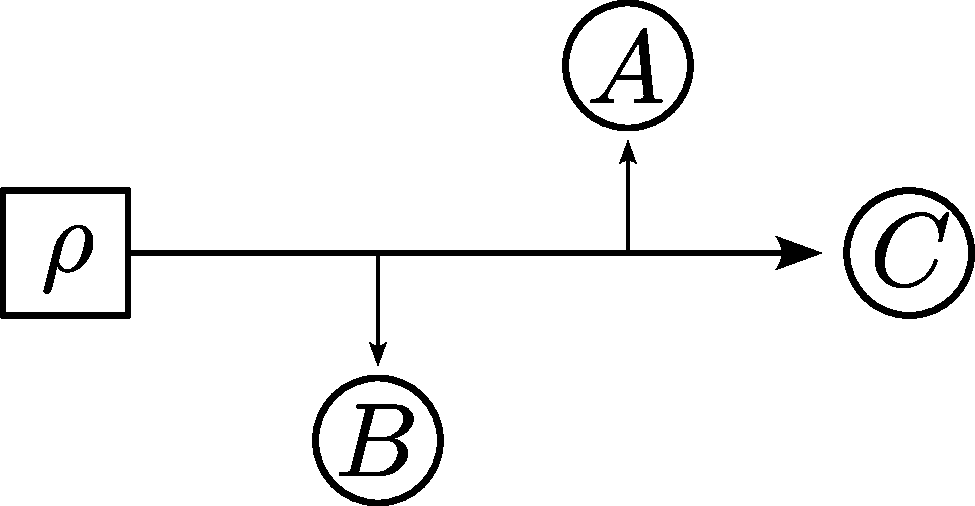
\includegraphics[scale=.3]{figs/wBAC.pdf}
				\end{figure}
				\vspace{1cm}
				
			\end{column}
		\end{columns}
		
	\end{frame}
	
	\begin{frame}{LG assumptions}
		
		\begin{columns}
			
			\begin{column}{0.5\textwidth}
				\textbf{Macrorealism}. A macroscopic object, which has available to it two or more macroscopically distinct states, is at any given time in a definite one of those states.

			\end{column}
			
			
			\begin{column}{0.5\textwidth}
				\textbf{Noninvasiveness of measurements}. It is possible in principle to determine which of these states the system is in without any effect on the state itself, or on the subsequent system dynamics.

				
			\end{column}
		\end{columns}
		
	\end{frame}
	
	\begin{frame}{Time order}
		
		Classical noninvasive measurements cannot depend on their order,
		\be
		\langle \mathcal A\mathcal B\mathcal C\rangle=\langle \mathcal B\mathcal A\mathcal C\rangle \label{orr}
		\ee
		with the first order $A\to B\to C$ and the second order $B\to A\to C$. In contrast, quantum correlations, even noninvasive, depend on the order,
		\be
		\langle \mathcal A\mathcal B\mathcal C\rangle- \langle \mathcal B\mathcal A\mathcal C\rangle=
		\langle [[A,B],C]\rangle/4.
		\ee
		
	\end{frame}

	\begin{frame}{Weak measurements}
		
		\begin{columns}
			\begin{column}{0.5\textwidth}
				
				\begin{itemize}
				
					\item Noninvassive, but not precise (requires large statistics)
					
					\item Still not known if these are pratcital to use.
					
					\item Capable of detecting nonclassical properties (like LG or time order violations).
					
					\item Naturally realized by weakly entangling (eg. fractional) gates.
					
				\end{itemize}
				
			\end{column}
			
			\begin{column}{0.5\textwidth}
				
				\begin{figure}
					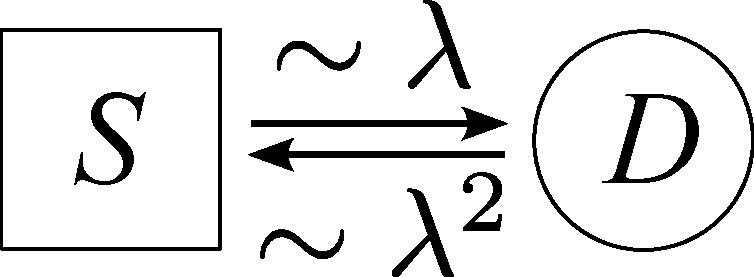
\includegraphics[width=\linewidth]{figs/wsch.pdf}
					\caption{The scheme of weak measurement. The system $S$ interacts with the ancillary
						detector $D$ which gains information from the weakly-measured system scaled by the measurement
						strength $\lambda$, while causing disturbance to the system of the
						order $\lambda^2$.}
					\label{weakscheme}
				\end{figure}
				\vspace{1cm}
				
			\end{column}
		\end{columns}
		
		
		
		
		
	\end{frame}
	
	\begin{frame}{Weak measurements}
		
		To construct their general family, we shall look into the construction of POVM,
		expressing Kraus operators by elements of a system-meter unitary transition $U$
		in the space $\mathcal H\otimes \mathcal H_M$, 
		\be
		K(a)=\langle a|U|\Omega\rangle\label{kra}
		\ee
		with the meter states $|\Omega\rangle$ and $|a\rangle$, assuming the meter initially in
		pure $|\Omega\rangle$ state, and measuring projectively $P_a=|a\rangle\langle a|$,
		calibrated to zero average bias for null detection,
		\be
		\langle a\rangle_\Omega=\int da\; |\langle a|\Omega\rangle|^2=0.\label{unbias}
		\ee
		The weak measurement can be defined by weakening $U\to U^\lambda$, with $\lambda \to 0$.
		
		
		
		
	\end{frame}

%%%%%%%%%%%%%%%%%%%%%%%%%%%%%%%%%%%%%%%%%%%%%%%
\section{Experiments}

	\begin{frame}{Overview}
		
		\begin{columns}
			\begin{column}{0.5\textwidth}
				
				\begin{enumerate}
					
					\item Single measurement scheme for time order and LG tests.
					
					\item 2 protocols realizing the measurement scheme.
					
					\item Tested on 6 devices (5 IBM + IonQ).
					
					\item Dichotomic measurements.
					
					\item Backed up by simulations.
					
				\end{enumerate}
				
				\textbf{Notation}
				\begin{itemize}
					\item We use \textit{mathcal} for weak measurements ($\mathcal{A}$ is $A$ measured weakly)
					\item $V_\theta=\exp(-i\theta V/2)=\cos(\theta/2)-iV\sin(\theta/2)$
				\end{itemize}
				
			\end{column}
			
			\begin{column}{0.5\textwidth}
				
				\begin{figure}
					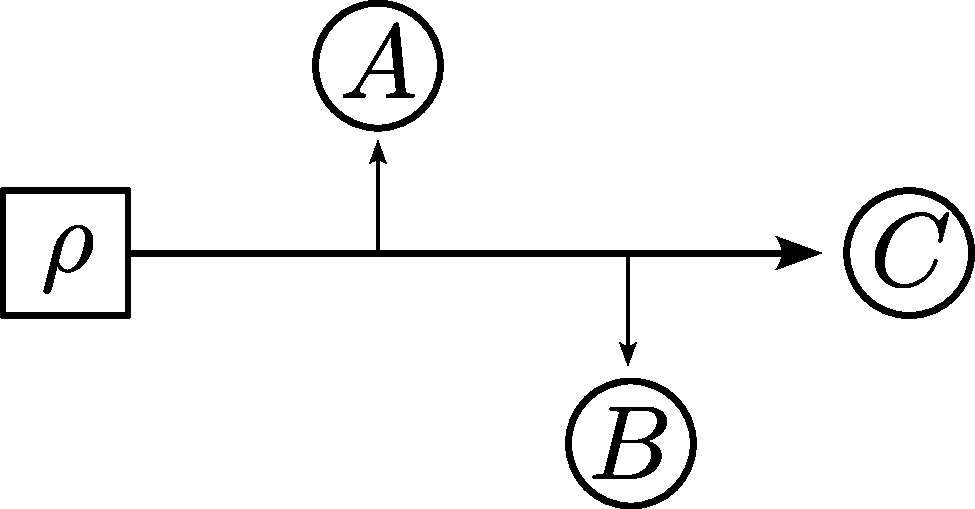
\includegraphics[scale=.3]{figs/wABC.pdf}\\
					\medskip
					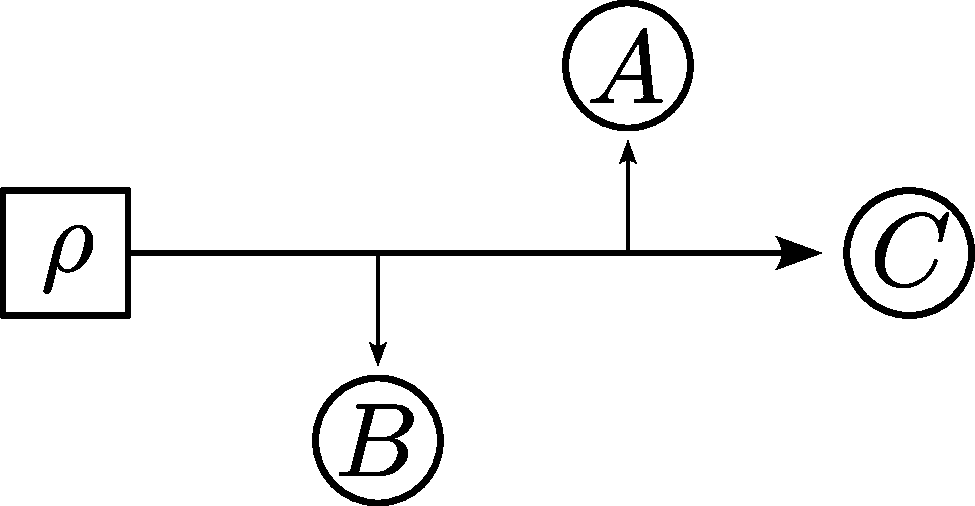
\includegraphics[scale=.3]{figs/wBAC.pdf}
				\end{figure}
				\vspace{1cm}
				
				
			\end{column}
		\end{columns}
		
	\end{frame}
	
	\begin{frame}
		\begin{figure}
			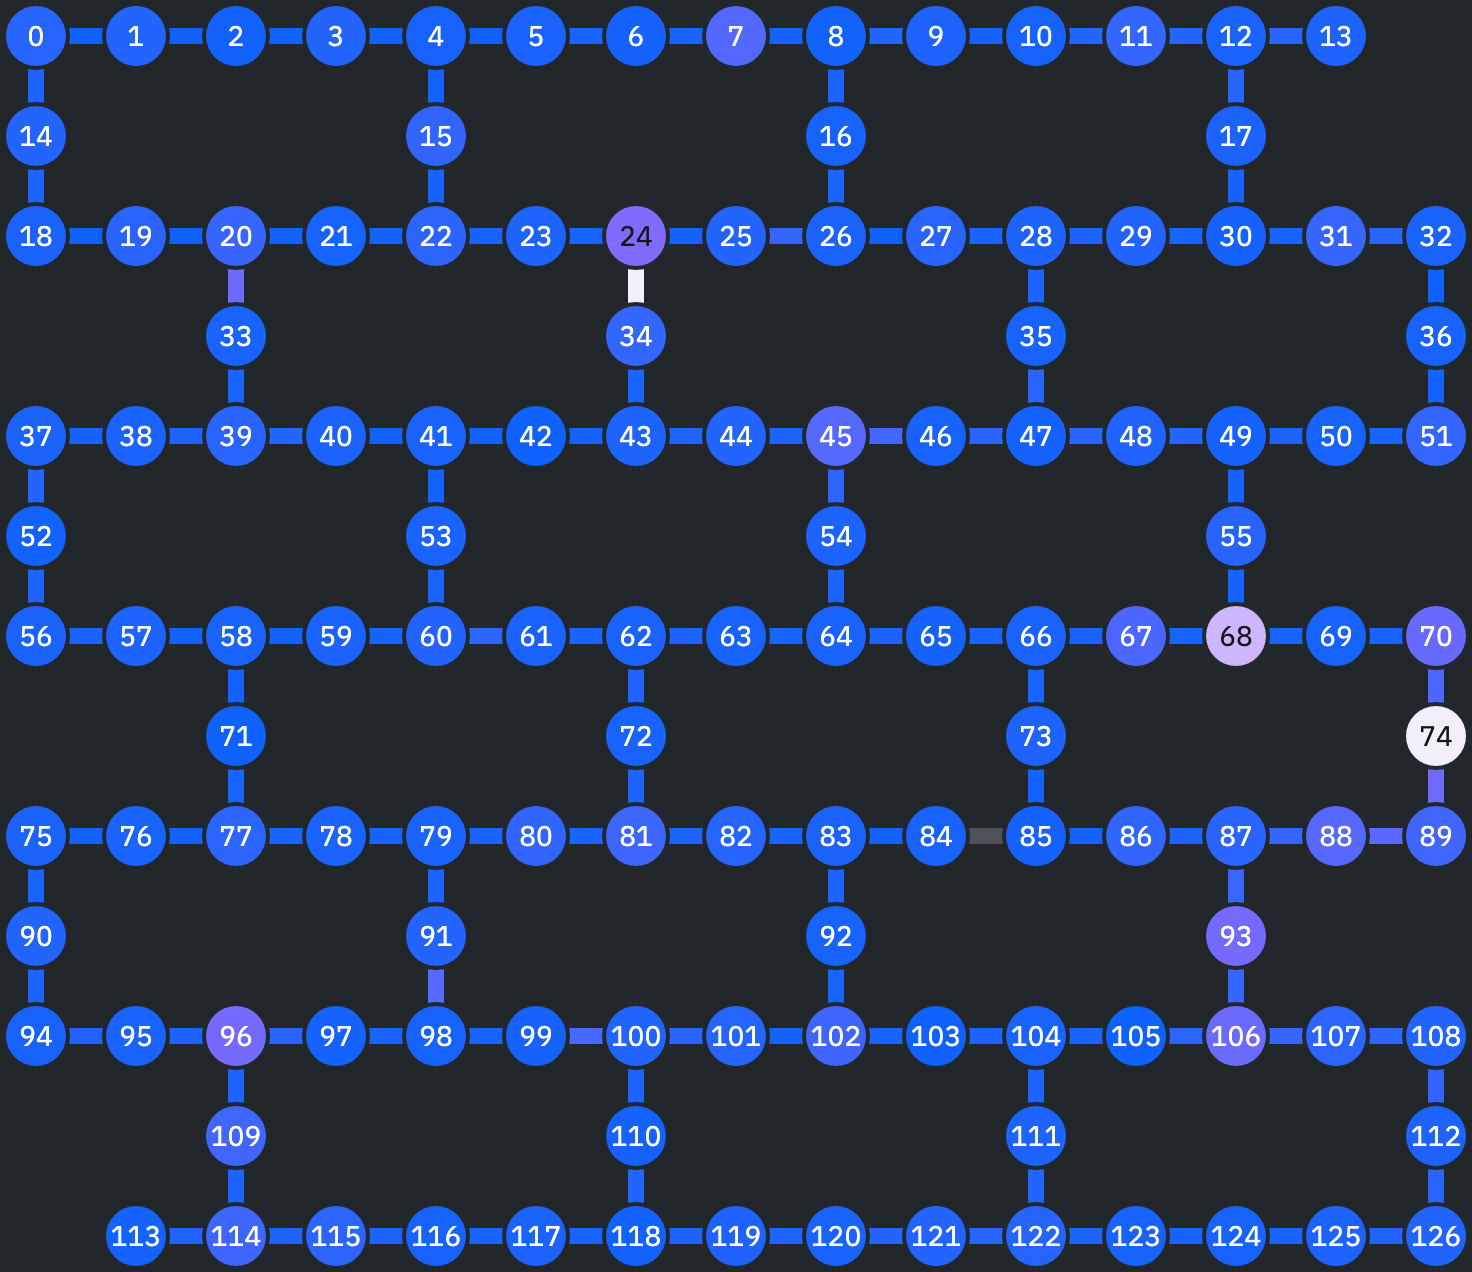
\includegraphics[scale=0.18]{figs/brisbane_map.png}
		\end{figure}
	\end{frame}

	\begin{frame}{Experimental setup}
		
		To realize weak measurement on a qubit, it must
		be entangled with an auxiliary meter qubit by a two-qubit operation/gate. We have
		implemented two different protocols of weak measurement:
		\vspace{0.2cm}
		\begin{columns}
			\hspace{0.2cm}
			\begin{column}{0.4\textwidth}
				\textbf{Protocol I}
				\begin{enumerate}
					
					\item The meter is close to the special state $\sim|\Omega\rangle$ for which
					applying the operation $V'$ does not affect the system, i.e.
					$V'|\psi\rangle|\Omega\rangle=|\psi\rangle|\Omega\rangle$ for an arbitrary
					$|\psi\rangle$.
					
					\item Single entangling gate needed.
					
				\end{enumerate}
				
			\end{column}
			
		
			\begin{column}{0.4\textwidth}
				\textbf{Protocol II}		
				\begin{enumerate}
					
					\item The constructed operation $U$ is $\sim 1$, i.e. close to identity.
					
					\item May require 2 entangling gates.
					
					\item Closer to explicit formulation of weak measurements.
					
				\end{enumerate}
				
				
			\end{column}
		\end{columns}
		
		
	\end{frame}
	
	\begin{frame}{Observables and inequalities}
		
		Selected observables:
		\begin{align*}
			&A=e^{i\pi/4}|+\rangle\langle -|+e^{-i\pi/4}|-\rangle\langle +|\nonumber\\
			&B=e^{-i\pi/4}|+\rangle\langle -|+e^{i\pi/4}|-\rangle\langle +|\nonumber\\
			&C=i|-\rangle\langle+|-i|+\rangle\langle -|
		\end{align*}
		Then 
		\begin{align*}
			&\langle \mathcal A\rangle=\langle\mathcal B\rangle=1/\sqrt{2}\nonumber\\
			&\langle \mathcal A\mathcal B\rangle=\langle \mathcal B\mathcal A\rangle=0,\nonumber\\
			&\langle \mathcal A\mathcal B\mathcal C\rangle=-\langle \mathcal B\mathcal A\mathcal C\rangle=1/2
		\end{align*}
		LG inequalities:
		\begin{align*}
			&\langle\mathcal A\rangle+\langle\mathcal B\rangle-\langle\mathcal A\mathcal B\rangle\leq 1\nonumber\\
			&\langle\mathcal A\rangle+\langle\mathcal B\rangle-\langle\mathcal B\mathcal A\rangle\leq 1
			\label{lgg}
		\end{align*}
		
	\end{frame}
	
	\begin{frame}{Protocol I overview}
		
		Protocol (I) is realized in the following way. We take
		\begin{align}
			&|\Omega_\theta\rangle=X_+Z_{\theta+\pi/2} X_+\ket 0=\nonumber\\
			&\sin(\theta/2+\pi/4)\ket 0+\cos(\theta/2+\pi/4)\ket 1,
		\end{align}
		apply $CX|\psi\Omega_\lambda\rangle$, assuming system state $\ket \psi $ and
		measure $Z\to\pm 1$ on the meter qubit. One can notice that we end up with the scheme
		for $A=\lambda Z$ with $\lambda=\sin(\theta)$, i.e. $\sqrt{2}K_\pm=\cos\theta/2+Z\sin\theta/2.$
		Instead of $CX$, the native gate on IBM Heron devices, like \texttt{ibm\_torino}, is $CZ$.
		 This enforces a slight modification of protocol (I) implementation.
		The prepared meter state is 
		\begin{align}
		|\Omega_\theta\rangle=ZX_+Z_{\theta+\pi} X_+\ket 0=\cos(\theta/2)\ket 0+\sin(\theta/2)\ket 1
		\end{align}
		instead, and one measures $X$.
	
	\end{frame}
	
	\begin{frame}{Protocol I with CX gate}
		
		\begin{figure}
		
			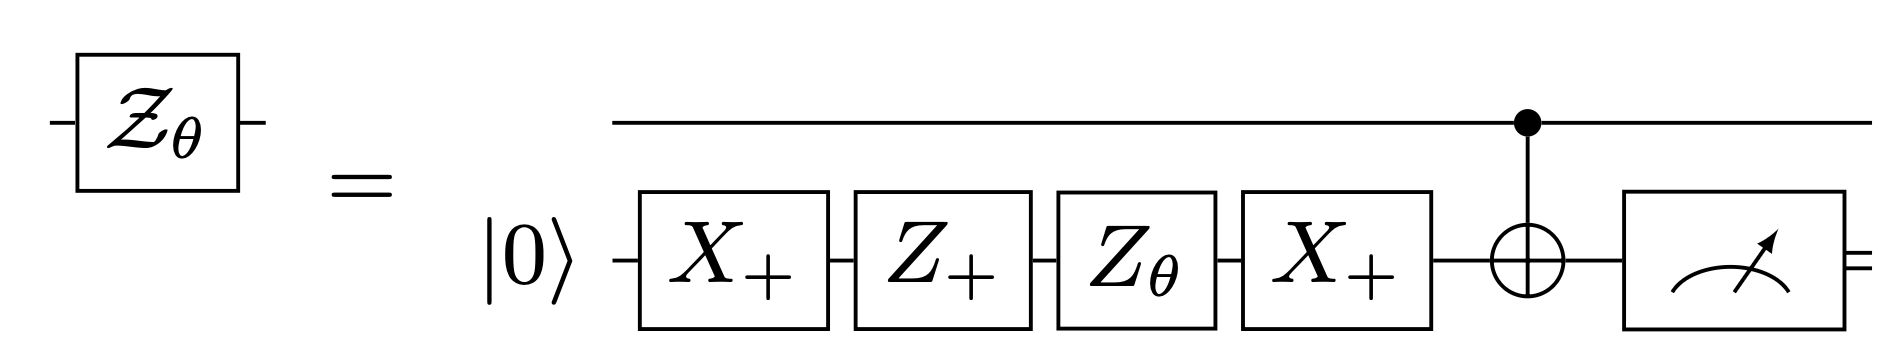
\includegraphics[width=\linewidth]{figs/p1_CX.png}
			
		\end{figure}
		
	\end{frame}
	
	\begin{frame}{Protocol I with CZ gate}
		
		\begin{figure}
			
			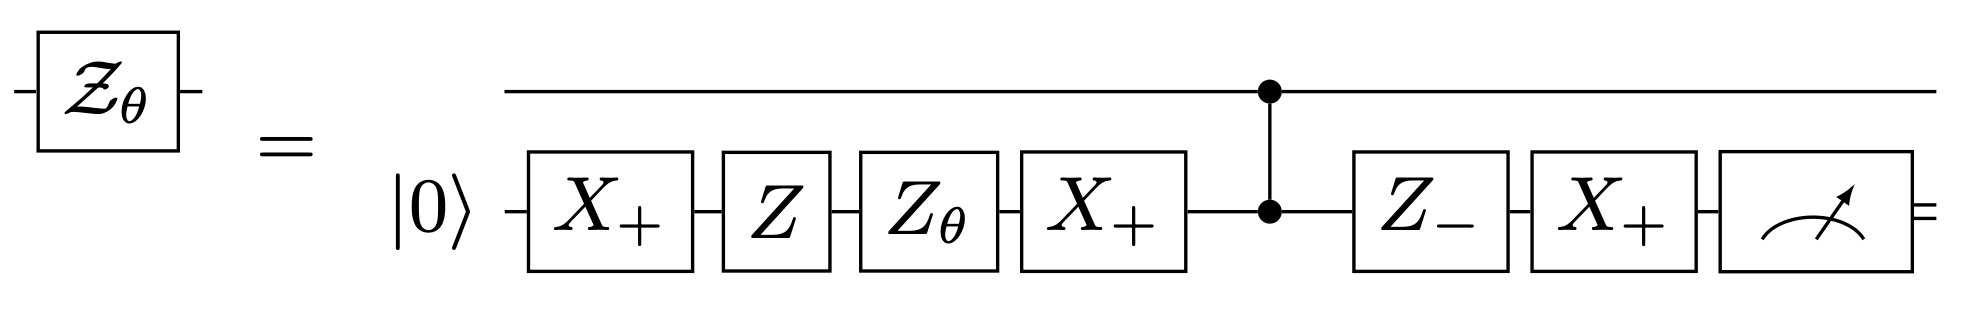
\includegraphics[width=\linewidth]{figs/p1_CZ.png}
			
		\end{figure}
		
	\end{frame}
	
	\begin{frame}{Protocol I with ECR gate}
		
		\begin{figure}
			
			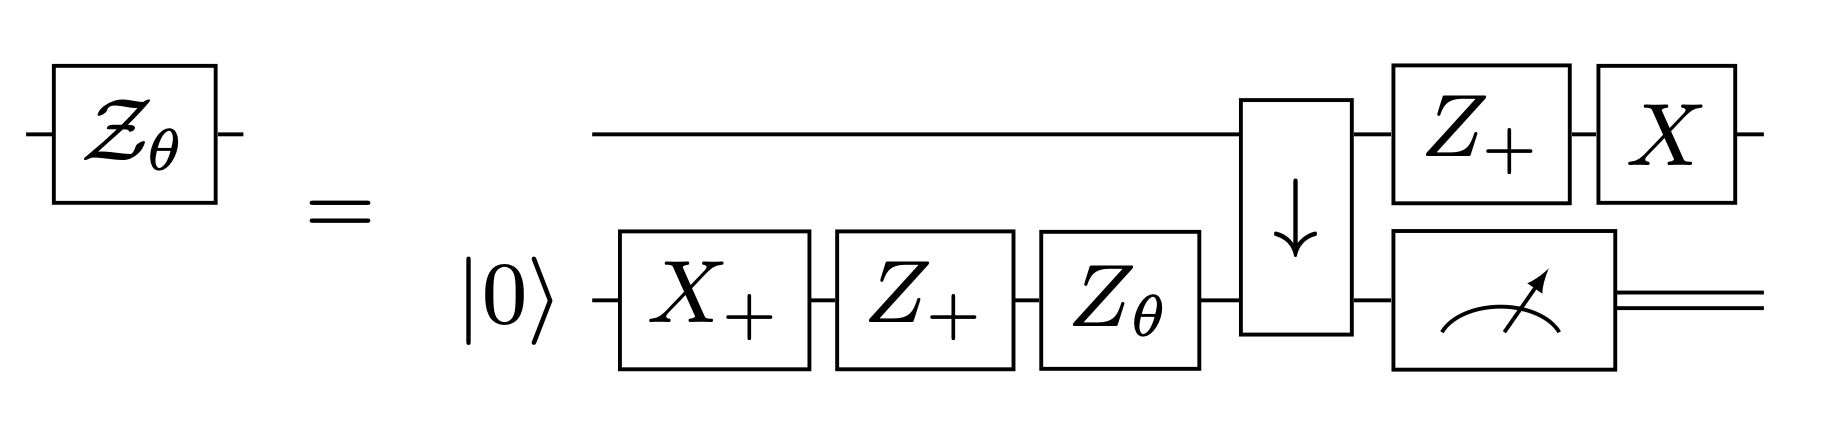
\includegraphics[width=\linewidth]{figs/p1_ECR.png}
			
		\end{figure}
		
	\end{frame}
	
	\begin{frame}{Protocol II overview}
		
		The protocol (II) needs an operation $\sim 1$ which is realized by two
		$ECR$ gates ($(ECR)(ECR) = 1$) with a small phase shift on the meter (target) qubit
		\begin{align}
			&(ZY)_\theta=II\cos(\theta/2)-iZY\sin(\theta/2)\nonumber\\
			&ECR_\downarrow(IZ_\theta)ECR_\downarrow
		\end{align}
		on IBM Eagle devices. It's similar for IBM Heron devices, where one uses two $CZ$ gates with the phase
		shift sandwiched by a pair of $ZX_+$. The meter qubit is initially in the state
		$|0\rangle$ and finally measured by $X=\pm 1$. It's possible by applying 
		$Y_-$ rotation before readout since $Y_+ZY_-=-iYZ=X$. The resulting POVM is identical to the protocol (I).
		
	\end{frame}
	
	\begin{frame}{Protocol II with CZ gates}
		
		\begin{figure}
			
			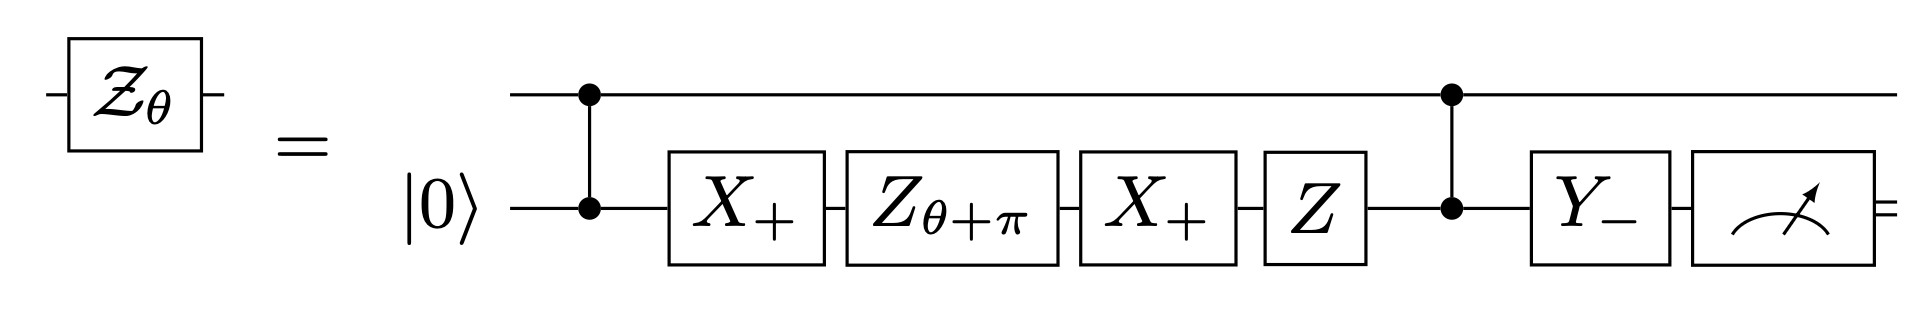
\includegraphics[width=\linewidth]{figs/p2_CZ.png}
			
		\end{figure}
		
	\end{frame}
	
	\begin{frame}{Protocol II with ECR gates}
		
		\begin{figure}
			
			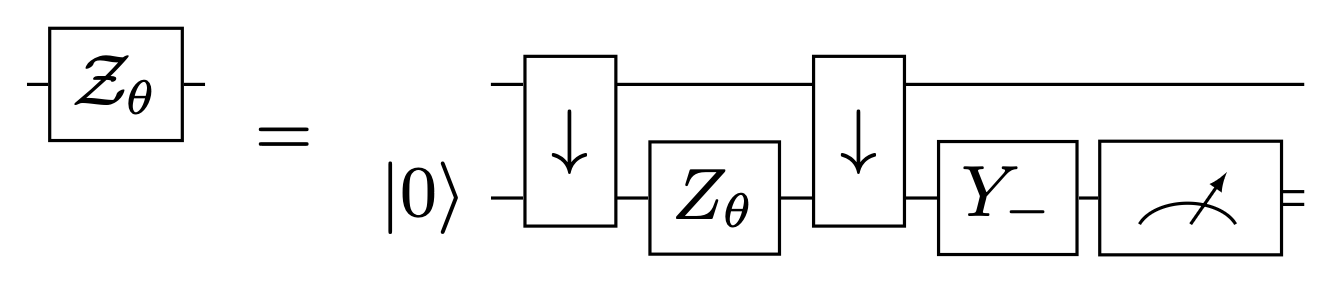
\includegraphics[width=\linewidth]{figs/p2_ECR.png}
			
		\end{figure}
		
	\end{frame}
	
	\begin{frame}{Protocol II with fractional ZZ$_\theta$ gates}
		
		\begin{figure}
			
			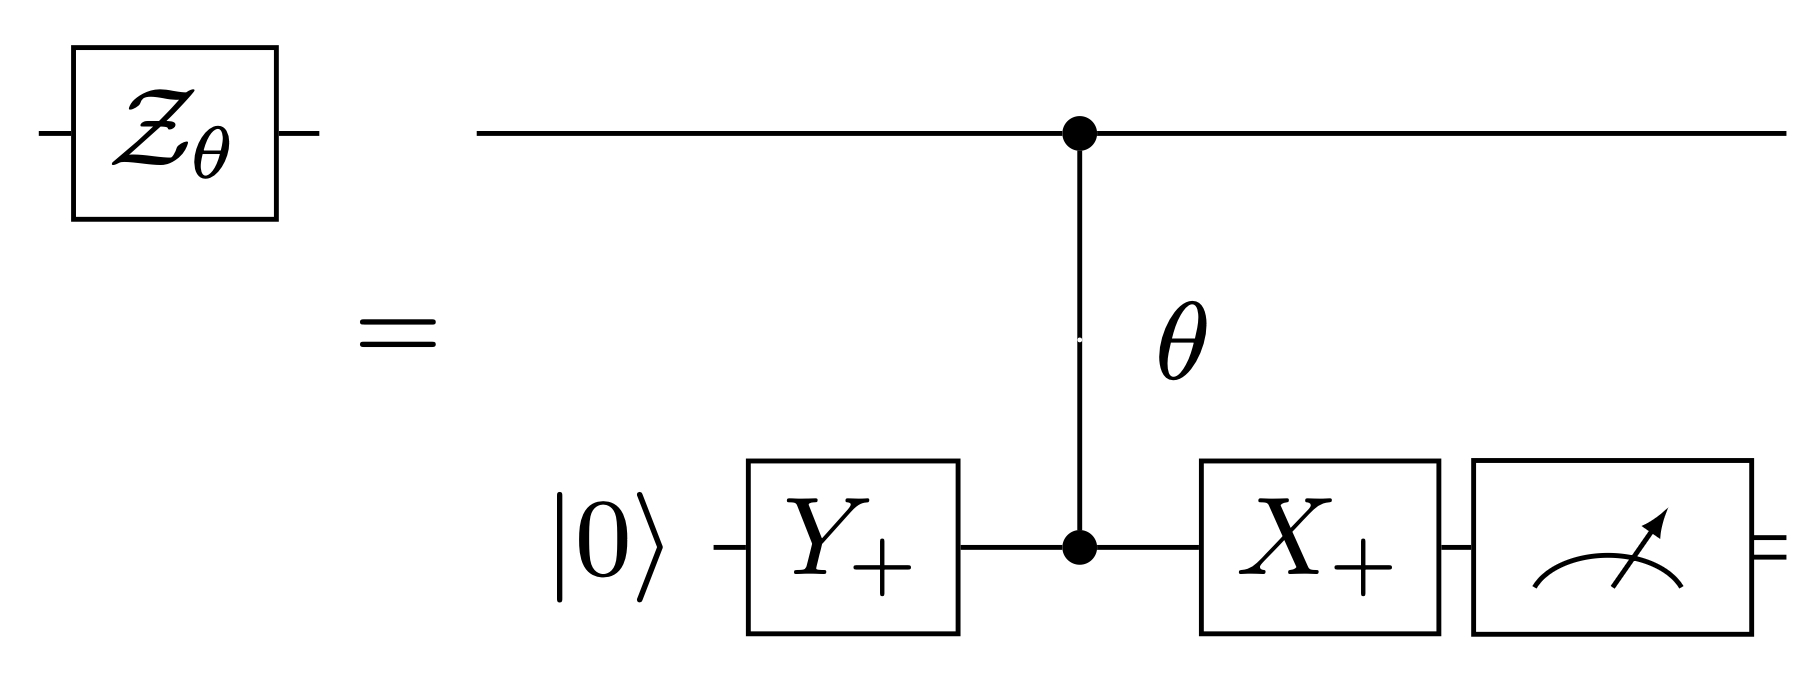
\includegraphics[width=0.8\linewidth]{figs/p2_ZZ.png}
			
		\end{figure}
		Fractional, symmetric $ZZ_\theta$ (native for IonQ devices)\\
		\begin{equation}
			\begin{pmatrix}
				e^{i\theta/2}&0&0&0\\
				0&e^{-i\theta/2}&0&0\\
				0&0&e^{-i\theta/2}&0\\
				0&0&0&e^{i\theta/2}
			\end{pmatrix}
		\end{equation}
		
	\end{frame}

%%%%%%%%%%%%%%%%%%%%%%%%%%%%%%%%%%%%%%%%%%%%%%%
\section{Results}
	
	\begin{frame}{LG violations on IBM}
		\vspace{-1cm}
		\begin{figure}[H]
			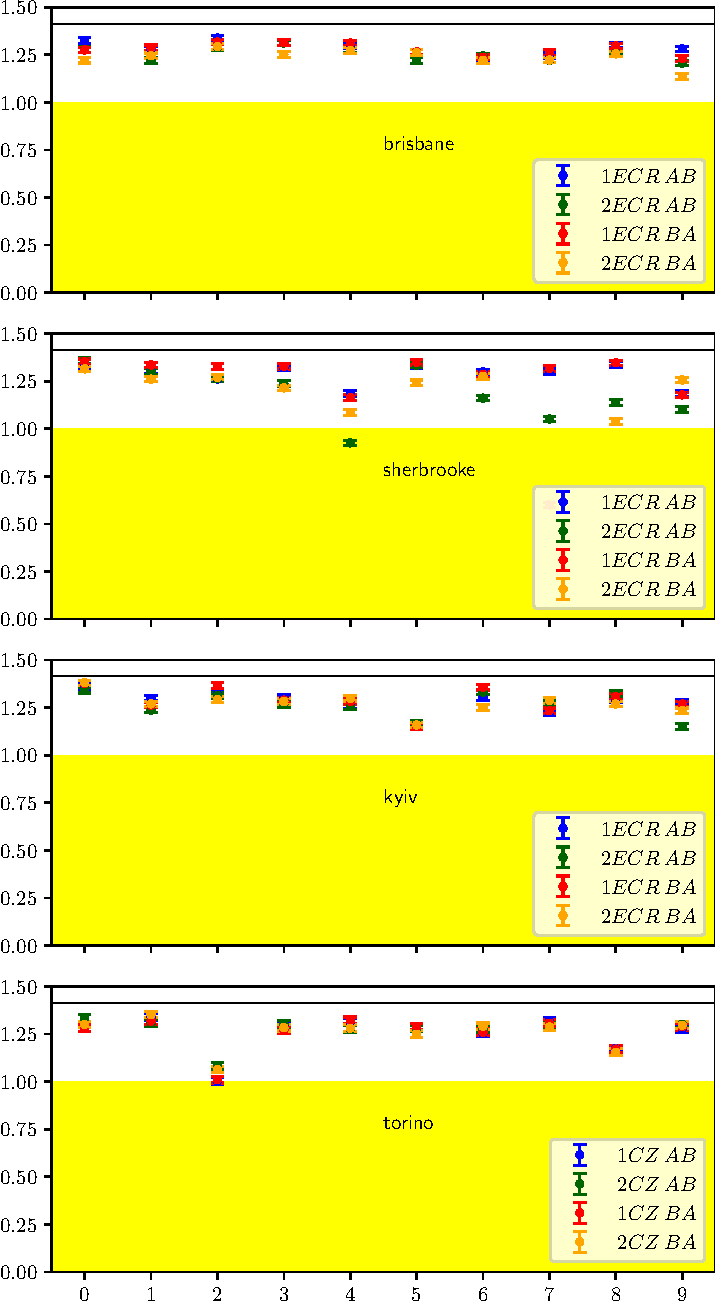
\includegraphics[scale=.3]{figs/lg.pdf}
			\hspace{1cm}
			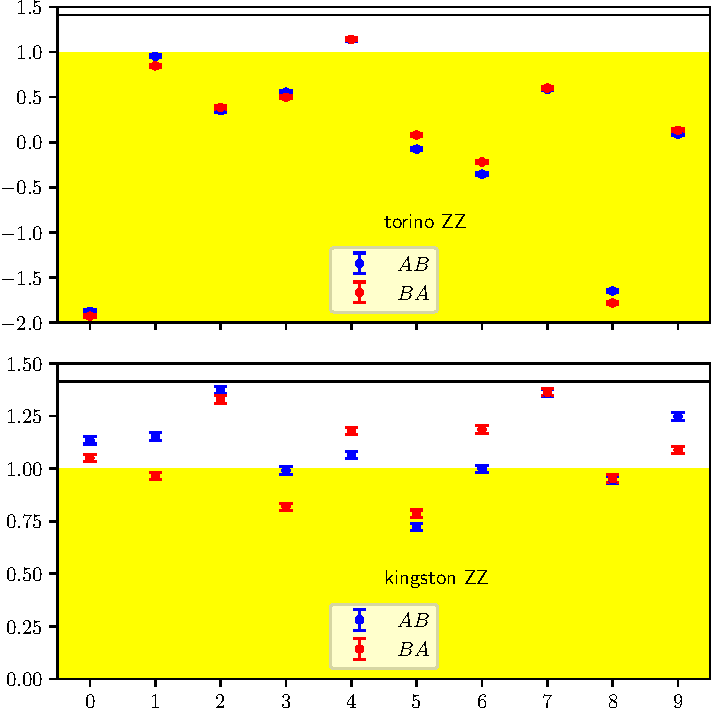
\includegraphics[scale=.5]{figs/lgzz.pdf}
		\end{figure}
	\end{frame}
	
	\begin{frame}{Time order correlations ($\langle ABC \rangle$ and $\langle BAC \rangle$) on IBM}
		
			\vspace{-1cm}
			\begin{figure}[H]
				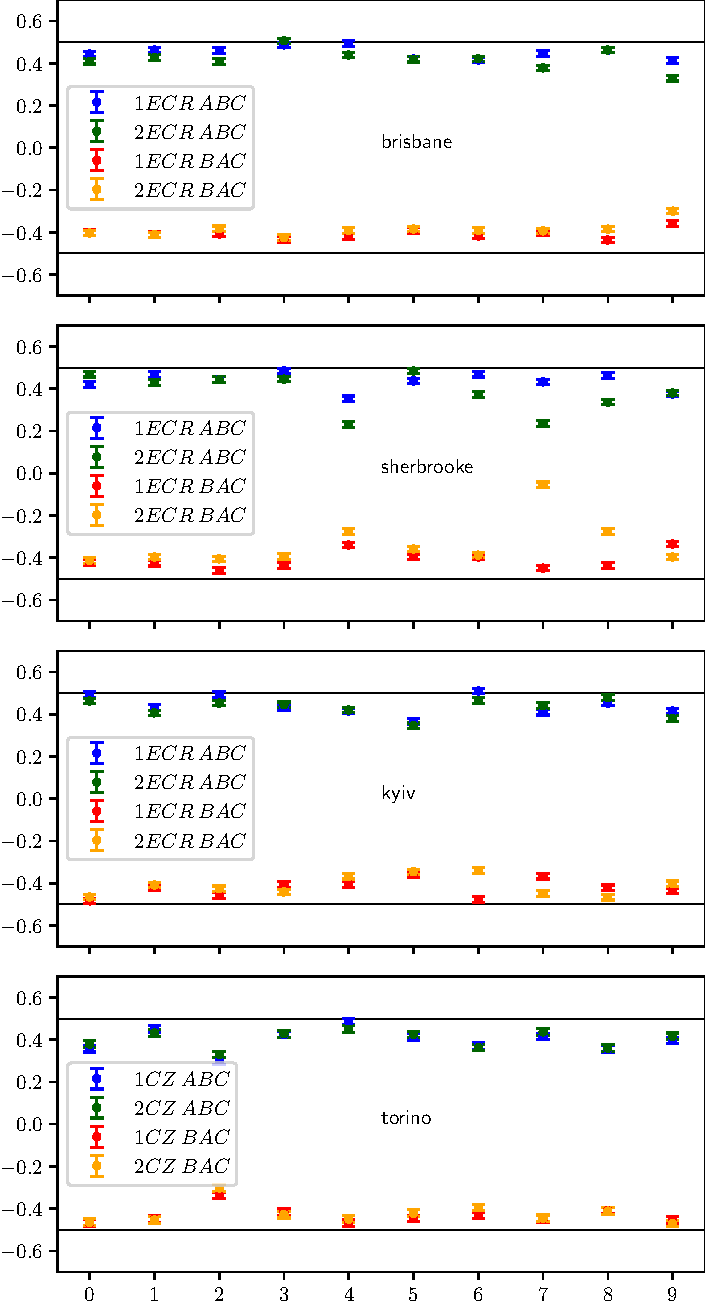
\includegraphics[scale=0.3]{figs/ABC.pdf}
				\hspace{1cm}
				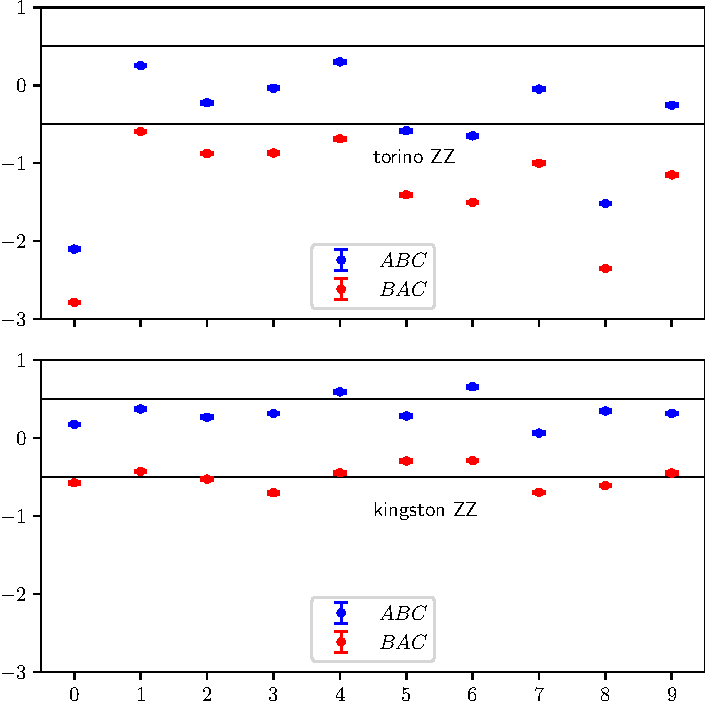
\includegraphics[scale=.5]{figs/ABCzz.pdf}
				\label{ABC}
			\end{figure}
	
	\end{frame}
	
	\begin{frame}{Time order violation on IBM}
		\vspace{-1cm}
		\begin{figure}[H]
			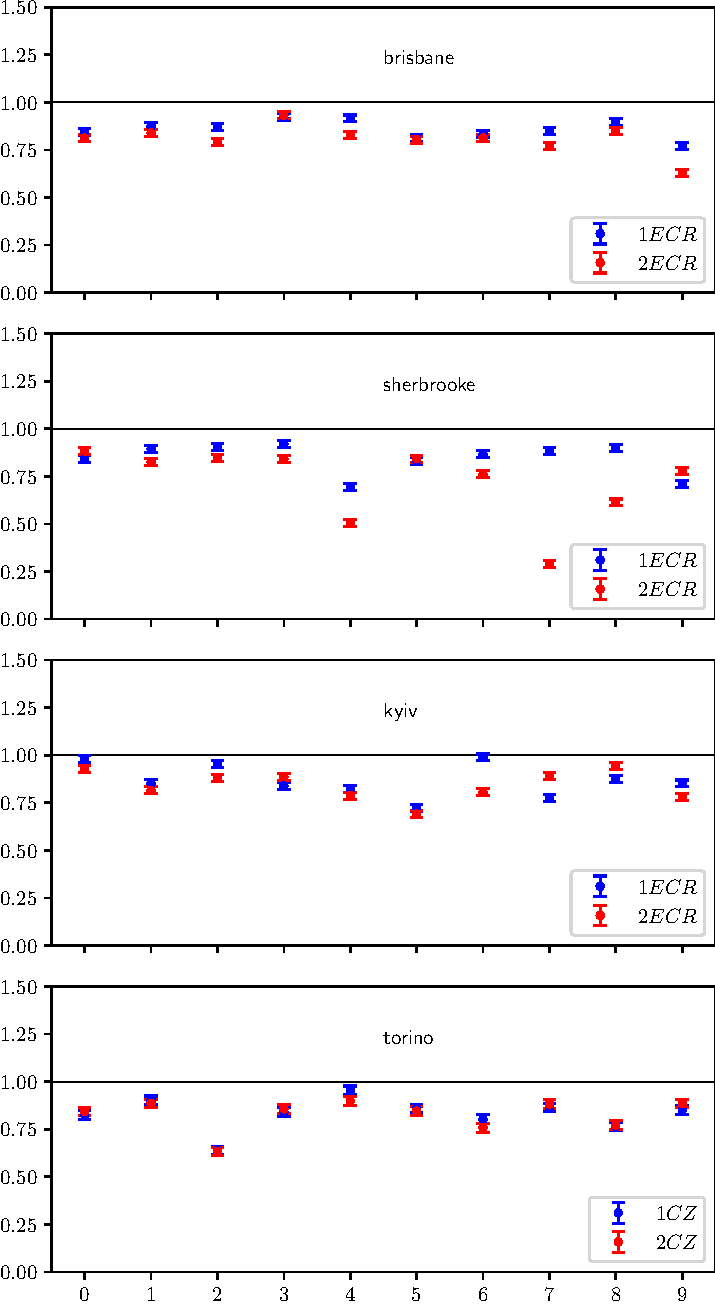
\includegraphics[scale=.3]{figs/order.pdf}
			\hspace{1cm}
			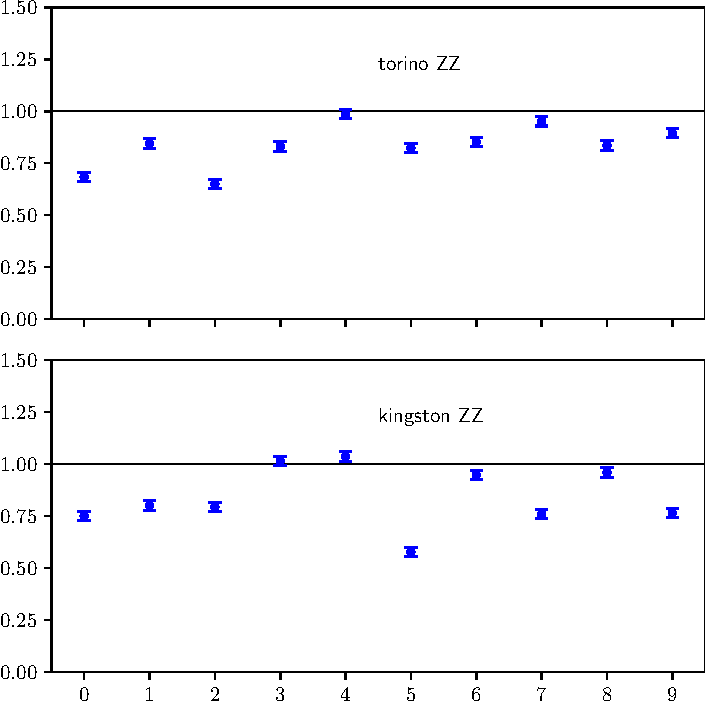
\includegraphics[scale=.5]{figs/orderzz.pdf}
		\end{figure}
	\end{frame}
	
	\begin{frame}{LG and time order tests on IonQ}
		
		\begin{columns}
			\begin{column}{0.5\textwidth}
				\tiny
				\begin{table}
					\begin{tabular}{*{3}{c}}
						quantity &value&error\\
						\hline
						LG$AB$&\textbf{1.583} & 0.025\\
						LG$BA$&\textbf{1.569} & 0.025\\
						order&\textbf{1.190} & 0.032\\
						$\langle ABC\rangle$&0.630& 0.022\\
						$\langle BAC\rangle$&-0.560& 0.022\\
						$\langle AB\rangle$&0.020&0.022\\
						$\langle BA\rangle$&0.004&0.022\\
						$\langle AbC\rangle$&-0.768&0.002\\
						$\langle bAC\rangle$&-0.786&0.002\\
						$\langle aBC\rangle$&0.790&0.002\\
						$\langle BaC\rangle$&0.783&0.002\\
						$\langle Ab\rangle$&0.799&0.002\\
						$\langle bA\rangle$&0.787&0.002\\
						$\langle aB\rangle$&0.790&0.002\\
						$\langle Ba\rangle$&0.800&0.002\\
						$\langle abC\rangle$&0.011&0.0002\\
						$\langle baC\rangle$&0.008&0.0002\\
						\hline
					\end{tabular}
					
					\label{tabi}
				\end{table}
				
			\end{column}
			
			\begin{column}{0.5\textwidth}
					
					\begin{itemize}

						\item Experiments done on IonQ Forte Enterprise 1 (all-to-all connectivity)
						
						\item Single entangling gate protocol
						
						\item Fractional gate (RZZ)
						
						\item Arbitrarily selected 3-qubit group (no differences between the qubits)
						
					\end{itemize}
				
			\end{column}
		\end{columns}
		
	\end{frame}
	
	\begin{frame}{Key takeaways}
		
		\begin{enumerate}
		
			\item LG inequality is violated on contemporary QCs, in most cases.

			\item Natural realization of weak measurements via fractional gates (RZZ) turned out to be worse than via full entangling gates (CX / CZ / ECR).
			
			\item ION QC seems to work better, but more experiments are needed to strengthen that claim.
			
		\end{enumerate}
		
	\end{frame}
	
%%%%%%%%%%%%%%%%%%%%%%%%%%%%%%%%%%%%%%%%%%%%
\section{Conclusion}

	\begin{frame}{Acknowledgements}
		The results have been created using IBM Quantum. The views expressed are those of the
		authors and do not reflect the official policy or position of the IBM Quantum team.
		TR gratefully acknowledges the funding support by program "{}Excellence
		initiative -- research university"{} for the AGH University in Krakow as well as the
		ARTIQ project: UMO-2021/01/2/ST6/00004 and ARTIQ/0004/2021. We thank 	
		Poznań Supercomputing and Networking Center	for the access to IBM Quantum Innovation Center.
	\end{frame}

	\begin{frame}{Thank you for your attention!}
	
		
	
		\begin{columns}
			
			\begin{column}{0.49\linewidth}
				
				\tiny
				
				\color{blue}{\Large \textbf{Find me!}}
				\begin{block}
					
					\begin{itemize}
						
						\item \url{rybotycki.tomasz@gmail.com}
						
						\item \url{https://twitter.com/TRybotycki}
						
						\item \url{https://orcid.org/0000-0003-2493-0459}
						
						\item \url{https://github.com/Tomev}
						
						\item \url{https://infosec.exchange/@tomev}
						
					\end{itemize}
					
				\end{block}
				
				\vspace{0.5cm}
				
				\color{blue}{\Large \textbf{QC Benchmarking}}
				\begin{block}

					\begin{itemize}
						\item \url{https://github.com/Tomev/IBMQ_Witness_Tests}
						\item arXiv:2112.07567
						\item arXiv:2301.03296 
						\item arXiv:2308.11246 
						\item arXiv:2312.13996  
						\item arXiv:2404.06792
						\item arXiv:2405.03013 
						\item arXiv:2405.18827  
						\item arXiv:2409.11348 
						\item LG manuscript coming soon!
					\end{itemize}
					
					
					
				\end{block}
				
				\vspace{1cm}
				
			\end{column} 
			
			\begin{column}{0.5\textwidth}
				\color{blue}{\Large \textbf{Outlook}}
				\begin{enumerate}
					
					\item We need more benchmarking tools for quantum computers.
					
					\item Weak measurements are efficient tools in QC benchmarking.
					
					\item Further experiments needed to confirm expected behavior on the ion-based QCs. 
					
					\item Further investigations needed for weak measurements with weak entanglement (pulses or fractional gates).
					
				\end{enumerate}
				
				\vspace{2cm}
				
			\end{column}
		
		\end{columns}
	
	\end{frame}
%%%%%%%%%%%%%%%%%%%%%%%%%%%%%%%%%%%%%%%%%%%%%%%%%%%%%%%%%%%%%%%%%%%%%%%%%%%%%%%%

\section{Bonus}
\subsection{Quantum Computers Benchmarking problems}

\begin{frame}{Benchmarking project issues}
	\begin{columns}
		\begin{column}{0.5\linewidth}
			\textbf{OOM problem}\vspace{0.5cm}
			
			When running a lot of circuits (for big statistics / different parameters) in one go, one can run into out-of-memory issues. Even when a single circuit execution is possible.\vspace{0.5cm}
			
			\textbf{Solution}\vspace{0.5cm}
			
			You can run each circuit in a separate process, this way the process memory is cleared along with the process, when the computations are done.
			
		\end{column}
		
		\begin{column}{0.5\linewidth}
			\textbf{Simulator access problem}\vspace{0.5cm}
			
			You can access \texttt{FakeBackends} but not with their full gatesets (fractional gates). \vspace{0.5cm}
			
			\textbf{Hack}\vspace{0.5cm}
			
			You can buy paid access for a dollar and create the simulator using \texttt{from\_backend} method. Never use up the credit for the computation!
			
			\vspace{1cm}
			
		\end{column}
	\end{columns}
\end{frame}

\end{document}
